
\documentclass[10pt,letterpaper]{article}
\usepackage[top=0.85in,left=2.75in,footskip=0.75in]{geometry}

% amsmath and amssymb packages, useful for mathematical formulas and symbols
\usepackage{amsmath,amssymb}

% Use adjustwidth environment to exceed column width (see example table in text)
\usepackage{changepage}

% textcomp package and marvosym package for additional characters
\usepackage{textcomp,marvosym}

% cite package, to clean up citations in the main text. Do not remove.
\usepackage{cite}

% Use nameref to cite supporting information files (see Supporting Information section for more info)
\usepackage{nameref,hyperref}

% line numbers
\usepackage[right]{lineno}

% ligatures disabled
\usepackage[nopatch=eqnum]{microtype}
\DisableLigatures[f]{encoding = *, family = * }

% color can be used to apply background shading to table cells only
%\usepackage[table]{xcolor}

% array package and thick rules for tables
\usepackage{array}

% create "+" rule type for thick vertical lines
\newcolumntype{+}{!{\vrule width 2pt}}

% create \thickcline for thick horizontal lines of variable length
\newlength\savedwidth
\newcommand\thickcline[1]{%
  \noalign{\global\savedwidth\arrayrulewidth\global\arrayrulewidth 2pt}%
  \cline{#1}%
  \noalign{\vskip\arrayrulewidth}%
  \noalign{\global\arrayrulewidth\savedwidth}%
}

% \thickhline command for thick horizontal lines that span the table
\newcommand\thickhline{\noalign{\global\savedwidth\arrayrulewidth\global\arrayrulewidth 2pt}%
\hline
\noalign{\global\arrayrulewidth\savedwidth}}


% Remove comment for double spacing
%\usepackage{setspace} 
%\doublespacing

% Text layout
\raggedright
\setlength{\parindent}{0.5cm}
\textwidth 5.25in 
\textheight 8.75in

% Bold the 'Fig #' in the caption and separate it from the title/caption with a period
% Captions will be left justified
\usepackage[aboveskip=1pt,labelfont=bf,labelsep=period,justification=raggedright,singlelinecheck=off]{caption}
\renewcommand{\figurename}{Fig}

% Use the PLoS provided BiBTeX style
\bibliographystyle{plos2015}

% Remove brackets from numbering in List of References
\makeatletter
\renewcommand{\@biblabel}[1]{\quad#1.}
\makeatother



% Header and Footer with logo
\usepackage{lastpage,fancyhdr,graphicx}
\usepackage{epstopdf}
\usepackage{lmodern}
%\pagestyle{myheadings}
\pagestyle{fancy}
\fancyhf{}
%\setlength{\headheight}{27.023pt}
%\lhead{\includegraphics[width=2.0in]{PLOS-submission.eps}}
\rfoot{\thepage/\pageref{LastPage}}
\renewcommand{\headrulewidth}{0pt}
\renewcommand{\footrule}{\hrule height 2pt \vspace{2mm}}
\fancyheadoffset[L]{2.25in}
\fancyfootoffset[L]{2.25in}
\lfoot{\today}

%% Include all macros below

\newcommand{\lorem}{{\bf LOREM}}
\newcommand{\ipsum}{{\bf IPSUM}}

%% END MACROS SECTION

%% personal packages and macro
%%% packages
\usepackage[utf8]{inputenc}        % allow utf-8 input
\usepackage[T1]{fontenc}           % use 8-bit T1 fonts
\usepackage[dvipsnames, table]{xcolor}
\usepackage{tabularx}
\usepackage{multirow}
\usepackage{pifont}
\usepackage{csvsimple}
\usepackage[font={small},textfont={it},labelfont={bf}]{caption}
\usepackage{subcaption}
\usepackage{graphicx}
\usepackage{url}                   % simple URL typesetting
\usepackage{booktabs}              % professional-quality tables
\usepackage{makecell}
\usepackage{amsfonts}              % blackboard math symbols
\usepackage{amsmath}
\usepackage{nicefrac}              % compact symbols for 1/2, etc.
\usepackage{microtype}             % microtypography
\usepackage{enumitem}
\usepackage[export]{adjustbox}


%not compatible with cite package
%\usepackage[natbib=true,style=nature,maxnames=999,maxcitenames=2,backend=biber]{biblatex}
%\addbibresource{references.bib}

%%% macros
\DeclareMathOperator*{\argmin}{arg\,min}
\newcommand{\indep}{\perp \!\!\! \perp}
\newtheorem{assumption}{Assumption}

\definecolor{dark_blue}{rgb}{0,0,.65}
\definecolor{dark_green}{rgb}{0,.5,.15}

\hypersetup{pdftex,  % needed for pdflatex
  breaklinks=true,  % so long urls are correctly broken across lines
  colorlinks=true,
  linkcolor=dark_blue,
  citecolor=dark_green,
}
\colorlet{P}{ForestGreen}
\colorlet{I}{MidnightBlue}
\colorlet{C}{YellowOrange}
\colorlet{O}{DarkOrchid}
\colorlet{T}{Gray}



\begin{document}
\vspace*{0.2in}

\section*{Supporting information}

% Include only the SI item label in the paragraph heading. Use the \nameref{label} command to cite SI items in the text.
\paragraph*{S1 Fig}
\label{apd:motivating_example}
{\bf Motivating example: Failure of predictive models to predict mortality
    from pretreatment variables.}
To illustrate how machine learning frameworks can fail to inform decision
making, we present a motivating example from MIMIC-IV. Using the same
population and covariates as in the main analysis (described in S1 Table), we train a predictive
model for 28-day mortality. We split the data into a training set (80\%) and a
test set (20\%). The training set uses the last measurements from the first 24
hours, whereas the validation set only uses the last measurements before the
administration of crystalloids. We split the train set into a train and a
validation set. We fit a HistGradientBoosting classifier
(\url{https://scikit-learn.org/stable/modules/ensemble.html\#histogram-based-gradient-boosting})
on the train set and evaluate the performance on the validation set and on the
test set. We see good area under the Precision-recall curve (PR AUC) on the
validation set, but a deterioration of 10 points on the test set (Fig
\ref{apd:fig:motivating_example_pr_auc}). The same is seen in Fig
\ref{apd:fig:motivating_example_roc_auc} when measuring performances with Area
Under the Curve of the Receiving Operator Characteristic (ROC AUC). On the
contrary, a model trained on pre-treatment features yields competitive
performances. This failure illustrates well the shortcuts on which predictive
models could rely to make predictions. A clinically useful predictive model
should support decision-making --in this case, addition of albumin to
crystalloids-- rather than maximizing predictive performance. In this example,
causal thinking would have helped to identify the bias introduced by
post-treatment features. In fact, these features should not be included in a
causal analysis since they are post-treatment colliders.

This kind of error might sound naive to a clinical expert but relying on
shortcuts --some of them being post-treatment variables-- is a common error.
Here, we detail some real use cases where machine learning fail in providing
useful predictions for decision-making. \cite{badgeley2019deep} use deep
learning to predict hip fracture using confounding patient and healthcare
variables. An example of such covariates shown by the authors is the triage of
patients before imaging that results in the model trying to predict the image
acquisition machine and rely on it to predict hip fracture.
\cite{obermeyer2019dissecting} describe the use of algorithm in US extra-care
programs. By equating care needs with previous care costs (in a pure
predictive fashion), the algorithm falsely conclude that Black patients are
healthier than equally white patients, since they do less money is spent on
them for a given level of need. Beyond Machine Learning, we also spotted the
inclusion of post-treatment variables in the development of the recent SCORE2
cardio-vascular risk score \cite{score22021score2}: \emph{Our risk models
    might have underestimated CVD risk be- cause data used to estimate multipliers
    were likely to include some people already on CVD prevention therapies (e.g.
    statins or anti- hypertensive medication}. This score might be used to inform
on the initiation of statins for primary prevention. But, relying on
post-treatment, it might under-discover patients who would benefit from
statins at screening time.


\begin{figure}[!h]
    \begin{subfigure}{\linewidth}
        \centering
        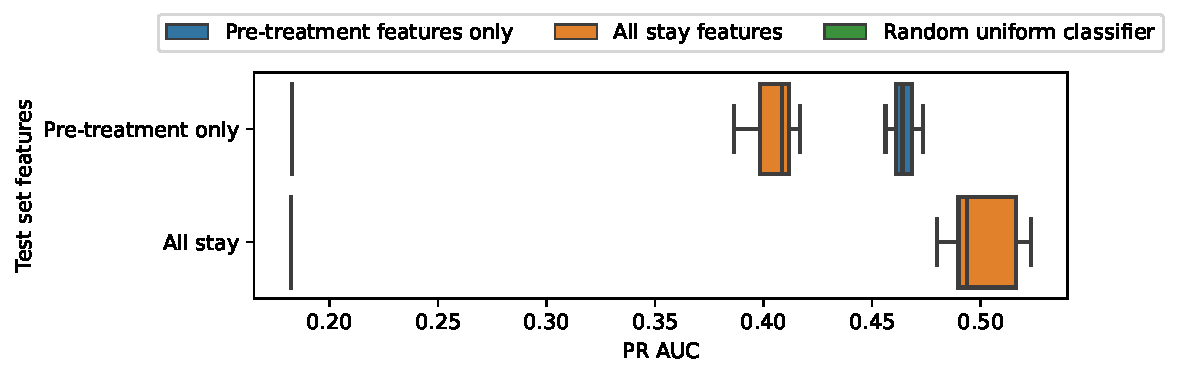
\includegraphics[width=0.8\linewidth]{img_supp_final/predictive_failure__pr_auc.pdf}
        \caption{Area under the Precision-Recall curve (PR\_AUC)}\label{apd:fig:motivating_example_pr_auc}
    \end{subfigure}
    \hfill
    \begin{subfigure}{\linewidth}
        \centering
        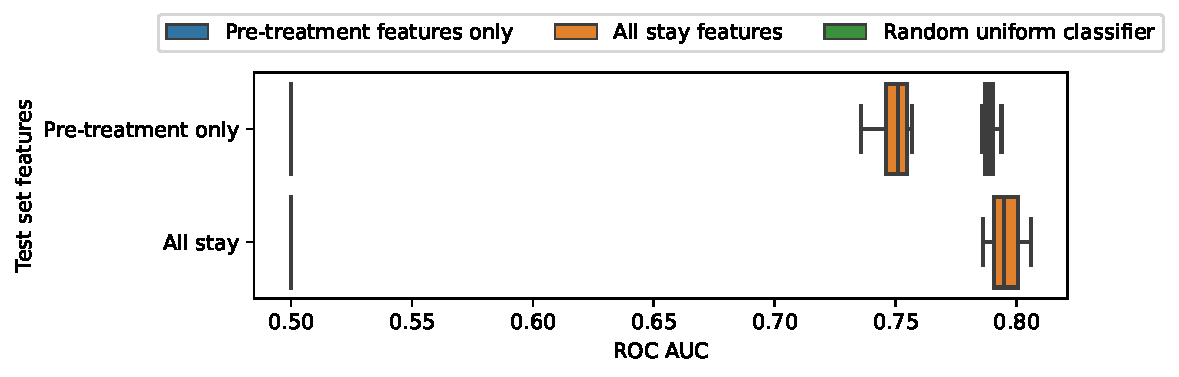
\includegraphics[width=0.8\linewidth]{img_supp_final/predictive_failure__roc_auc.pdf}
        \caption{Area under the Receiving Operator Characteristic (ROC\_AUC)}\label{apd:fig:motivating_example_roc_auc}
    \end{subfigure}
    \caption{\textbf{Failure to predict 28-day mortality from a model fitted on
            pre-treatment variables.}\\The model is trained on the last features from
        the whole stay and tested on two validation sets: one with all stay
        features and one with last features before crystalloids administration
        (Pre-treatment only). The all-stay model performance markedly decreases in
        the pre-treatment only dataset.}\label{apd:fig:motivating_example}
\end{figure}
\clearpage

\bibliography{references}

\end{document}
